%choose template: (un)comment all 5 lines:

%Template 1: IEEE (for Engineer's Internship Report, Seminar Paper, Researcher's Internship Report)
\documentclass[journal]{IEEEtran}
\usepackage{ifthen}
\newboolean{isIEEETemplate}\setboolean{isIEEETemplate}{true}
\newboolean{isArticleTemplate}\setboolean{isArticleTemplate}{false}
\newboolean{isReportTemplate}\setboolean{isReportTemplate}{false}


%%Template 2: scrartcl (for Engineer's Internship Report, Seminar Paper, Researcher's Internship Report)
%\documentclass[a4paper, 10pt, DIV10, pointlessnumbers]{scrartcl}
%\usepackage{ifthen}
%\newboolean{isIEEETemplate}\setboolean{isIEEETemplate}{false}
%\newboolean{isArticleTemplate}\setboolean{isArticleTemplate}{true}
%\newboolean{isReportTemplate}\setboolean{isReportTemplate}{false}


%%Template 3: scrreprt (for Bachelor Thesis, Master Thesis)
%\documentclass[a4paper, 10pt, DIV10, pointlessnumbers, appendixprefix=true]{scrreprt}
%\usepackage{ifthen}
%\newboolean{isIEEETemplate}\setboolean{isIEEETemplate}{false}
%\newboolean{isArticleTemplate}\setboolean{isArticleTemplate}{false}
%\newboolean{isReportTemplate}\setboolean{isReportTemplate}{true}




% *** KOMA SCRIPT OPTIONS ***

\ifthenelse{\boolean{isReportTemplate}}{
%	\numberwithin{figure}{chapter}
%	\numberwithin{table}{chapter}
%	\numberwithin{equation}{chapter}
}{}

\ifthenelse{\boolean{isArticleTemplate} \OR \boolean{isReportTemplate}}{
	\setkomafont{captionlabel}{\sffamily\bfseries}
%	\renewcommand{\figurename}{Fig.}
%	\renewcommand{\tablename}{Tab.}
}{}




% Some very useful LaTeX packages include:
% (uncomment the ones you want to load)


% *** MISC UTILITY PACKAGES ***
%
%\usepackage{ifpdf}
% Heiko Oberdiek's ifpdf.sty is very useful if you need conditional
% compilation based on whether the output is pdf or dvi.
% usage:
% \ifpdf
%   % pdf code
% \else
%   % dvi code
% \fi
% The latest version of ifpdf.sty can be obtained from:
% http://www.ctan.org/pkg/ifpdf
% Also, note that IEEEtran.cls V1.7 and later provides a builtin
% \ifCLASSINFOpdf conditional that works the same way.
% When switching from latex to pdflatex and vice-versa, the compiler may
% have to be run twice to clear warning/error messages.






% *** CITATION PACKAGES ***
%
\usepackage{cite}
% cite.sty was written by Donald Arseneau
% V1.6 and later of IEEEtran pre-defines the format of the cite.sty package
% \cite{} output to follow that of the IEEE. Loading the cite package will
% result in citation numbers being automatically sorted and properly
% "compressed/ranged". e.g., [1], [9], [2], [7], [5], [6] without using
% cite.sty will become [1], [2], [5]--[7], [9] using cite.sty. cite.sty's
% \cite will automatically add leading space, if needed. Use cite.sty's
% noadjust option (cite.sty V3.8 and later) if you want to turn this off
% such as if a citation ever needs to be enclosed in parenthesis.
% cite.sty is already installed on most LaTeX systems. Be sure and use
% version 5.0 (2009-03-20) and later if using hyperref.sty.
% The latest version can be obtained at:
% http://www.ctan.org/pkg/cite
% The documentation is contained in the cite.sty file itself.






% *** GRAPHICS RELATED PACKAGES ***
%
\ifCLASSINFOpdf
  \usepackage[pdftex]{graphicx}
  % declare the path(s) where your graphic files are
  % \graphicspath{{../pdf/}{../jpeg/}}
  % and their extensions so you won't have to specify these with
  % every instance of \includegraphics
  % \DeclareGraphicsExtensions{.pdf,.jpeg,.png}
\else
  % or other class option (dvipsone, dvipdf, if not using dvips). graphicx
  % will default to the driver specified in the system graphics.cfg if no
  % driver is specified.
  % \usepackage[dvips]{graphicx}
  % declare the path(s) where your graphic files are
  % \graphicspath{{../eps/}}
  % and their extensions so you won't have to specify these with
  % every instance of \includegraphics
  % \DeclareGraphicsExtensions{.eps}
\fi
% graphicx was written by David Carlisle and Sebastian Rahtz. It is
% required if you want graphics, photos, etc. graphicx.sty is already
% installed on most LaTeX systems. The latest version and documentation
% can be obtained at: 
% http://www.ctan.org/pkg/graphicx
% Another good source of documentation is "Using Imported Graphics in
% LaTeX2e" by Keith Reckdahl which can be found at:
% http://www.ctan.org/pkg/epslatex
%
% latex, and pdflatex in dvi mode, support graphics in encapsulated
% postscript (.eps) format. pdflatex in pdf mode supports graphics
% in .pdf, .jpeg, .png and .mps (metapost) formats. Users should ensure
% that all non-photo figures use a vector format (.eps, .pdf, .mps) and
% not a bitmapped formats (.jpeg, .png). The IEEE frowns on bitmapped formats
% which can result in "jaggedy"/blurry rendering of lines and letters as
% well as large increases in file sizes.
%
% You can find documentation about the pdfTeX application at:
% http://www.tug.org/applications/pdftex





% *** MATH PACKAGES ***
%
\usepackage{amsmath}
% A popular package from the American Mathematical Society that provides
% many useful and powerful commands for dealing with mathematics.
%
% Note that the amsmath package sets \interdisplaylinepenalty to 10000
% thus preventing page breaks from occurring within multiline equations. Use:
\interdisplaylinepenalty=2500
% after loading amsmath to restore such page breaks as IEEEtran.cls normally
% does. amsmath.sty is already installed on most LaTeX systems. The latest
% version and documentation can be obtained at:
% http://www.ctan.org/pkg/amsmath





% *** SPECIALIZED LIST PACKAGES ***
%
%\usepackage{algorithmic}
% algorithmic.sty was written by Peter Williams and Rogerio Brito.
% This package provides an algorithmic environment fo describing algorithms.
% You can use the algorithmic environment in-text or within a figure
% environment to provide for a floating algorithm. Do NOT use the algorithm
% floating environment provided by algorithm.sty (by the same authors) or
% algorithm2e.sty (by Christophe Fiorio) as the IEEE does not use dedicated
% algorithm float types and packages that provide these will not provide
% correct IEEE style captions. The latest version and documentation of
% algorithmic.sty can be obtained at:
% http://www.ctan.org/pkg/algorithms
% Also of interest may be the (relatively newer and more customizable)
% algorithmicx.sty package by Szasz Janos:
% http://www.ctan.org/pkg/algorithmicx




% *** ALIGNMENT PACKAGES ***
%
%\usepackage{array}
% Frank Mittelbach's and David Carlisle's array.sty patches and improves
% the standard LaTeX2e array and tabular environments to provide better
% appearance and additional user controls. As the default LaTeX2e table
% generation code is lacking to the point of almost being broken with
% respect to the quality of the end results, all users are strongly
% advised to use an enhanced (at the very least that provided by array.sty)
% set of table tools. array.sty is already installed on most systems. The
% latest version and documentation can be obtained at:
% http://www.ctan.org/pkg/array


% IEEEtran contains the IEEEeqnarray family of commands that can be used to
% generate multiline equations as well as matrices, tables, etc., of high
% quality.




% *** SUBFIGURE PACKAGES ***
%\ifCLASSOPTIONcompsoc
%  \usepackage[caption=false,font=normalsize,labelfont=sf,textfont=sf]{subfig}
%\else
%  \usepackage[caption=false,font=footnotesize]{subfig}
%\fi
% subfig.sty, written by Steven Douglas Cochran, is the modern replacement
% for subfigure.sty, the latter of which is no longer maintained and is
% incompatible with some LaTeX packages including fixltx2e. However,
% subfig.sty requires and automatically loads Axel Sommerfeldt's caption.sty
% which will override IEEEtran.cls' handling of captions and this will result
% in non-IEEE style figure/table captions. To prevent this problem, be sure
% and invoke subfig.sty's "caption=false" package option (available since
% subfig.sty version 1.3, 2005/06/28) as this is will preserve IEEEtran.cls
% handling of captions.
% Note that the Computer Society format requires a larger sans serif font
% than the serif footnote size font used in traditional IEEE formatting
% and thus the need to invoke different subfig.sty package options depending
% on whether compsoc mode has been enabled.
%
% The latest version and documentation of subfig.sty can be obtained at:
% http://www.ctan.org/pkg/subfig




% *** FLOAT PACKAGES ***
%
%\usepackage{fixltx2e}
% fixltx2e, the successor to the earlier fix2col.sty, was written by
% Frank Mittelbach and David Carlisle. This package corrects a few problems
% in the LaTeX2e kernel, the most notable of which is that in current
% LaTeX2e releases, the ordering of single and double column floats is not
% guaranteed to be preserved. Thus, an unpatched LaTeX2e can allow a
% single column figure to be placed prior to an earlier double column
% figure.
% Be aware that LaTeX2e kernels dated 2015 and later have fixltx2e.sty's
% corrections already built into the system in which case a warning will
% be issued if an attempt is made to load fixltx2e.sty as it is no longer
% needed.
% The latest version and documentation can be found at:
% http://www.ctan.org/pkg/fixltx2e


%\usepackage{stfloats}
% stfloats.sty was written by Sigitas Tolusis. This package gives LaTeX2e
% the ability to do double column floats at the bottom of the page as well
% as the top. (e.g., "\begin{figure*}[!b]" is not normally possible in
% LaTeX2e). It also provides a command:
%\fnbelowfloat
% to enable the placement of footnotes below bottom floats (the standard
% LaTeX2e kernel puts them above bottom floats). This is an invasive package
% which rewrites many portions of the LaTeX2e float routines. It may not work
% with other packages that modify the LaTeX2e float routines. The latest
% version and documentation can be obtained at:
% http://www.ctan.org/pkg/stfloats
% Do not use the stfloats baselinefloat ability as the IEEE does not allow
% \baselineskip to stretch. Authors submitting work to the IEEE should note
% that the IEEE rarely uses double column equations and that authors should try
% to avoid such use. Do not be tempted to use the cuted.sty or midfloat.sty
% packages (also by Sigitas Tolusis) as the IEEE does not format its papers in
% such ways.
% Do not attempt to use stfloats with fixltx2e as they are incompatible.
% Instead, use Morten Hogholm'a dblfloatfix which combines the features
% of both fixltx2e and stfloats:
%
% \usepackage{dblfloatfix}
% The latest version can be found at:
% http://www.ctan.org/pkg/dblfloatfix




%\ifCLASSOPTIONcaptionsoff
%  \usepackage[nomarkers]{endfloat}
% \let\MYoriglatexcaption\caption
% \renewcommand{\caption}[2][\relax]{\MYoriglatexcaption[#2]{#2}}
%\fi
% endfloat.sty was written by James Darrell McCauley, Jeff Goldberg and 
% Axel Sommerfeldt. This package may be useful when used in conjunction with 
% IEEEtran.cls'  captionsoff option. Some IEEE journals/societies require that
% submissions have lists of figures/tables at the end of the paper and that
% figures/tables without any captions are placed on a page by themselves at
% the end of the document. If needed, the draftcls IEEEtran class option or
% \CLASSINPUTbaselinestretch interface can be used to increase the line
% spacing as well. Be sure and use the nomarkers option of endfloat to
% prevent endfloat from "marking" where the figures would have been placed
% in the text. The two hack lines of code above are a slight modification of
% that suggested by in the endfloat docs (section 8.4.1) to ensure that
% the full captions always appear in the list of figures/tables - even if
% the user used the short optional argument of \caption[]{}.
% IEEE papers do not typically make use of \caption[]'s optional argument,
% so this should not be an issue. A similar trick can be used to disable
% captions of packages such as subfig.sty that lack options to turn off
% the subcaptions:
% For subfig.sty:
% \let\MYorigsubfloat\subfloat
% \renewcommand{\subfloat}[2][\relax]{\MYorigsubfloat[]{#2}}
% However, the above trick will not work if both optional arguments of
% the \subfloat command are used. Furthermore, there needs to be a
% description of each subfigure *somewhere* and endfloat does not add
% subfigure captions to its list of figures. Thus, the best approach is to
% avoid the use of subfigure captions (many IEEE journals avoid them anyway)
% and instead reference/explain all the subfigures within the main caption.
% The latest version of endfloat.sty and its documentation can obtained at:
% http://www.ctan.org/pkg/endfloat
%
% The IEEEtran \ifCLASSOPTIONcaptionsoff conditional can also be used
% later in the document, say, to conditionally put the References on a 
% page by themselves.




% *** PDF, URL AND HYPERLINK PACKAGES ***
%
\usepackage{url}
\usepackage[hyphens]{url}
\renewcommand{\UrlBreaks}{\do\/\do\a\do\b\do\c\do\d\do\e\do\f\do\g\do\h\do\i\do\j\do\k\do\l\do\m\do\n\do\o\do\p\do\q\do\r\do\s\do\t\do\u\do\v\do\w\do\x\do\y\do\z\do\A\do\B\do\C\do\D\do\E\do\F\do\G\do\H\do\I\do\J\do\K\do\L\do\M\do\N\do\O\do\P\do\Q\do\R\do\S\do\T\do\U\do\V\do\W\do\X\do\Y\do\Z}
%\usepackage[hyphenbreaks]{breakurl}
\urlstyle{same}
\usepackage{hyperref}
% url.sty was written by Donald Arseneau. It provides better support for
% handling and breaking URLs. url.sty is already installed on most LaTeX
% systems. The latest version and documentation can be obtained at:
% http://www.ctan.org/pkg/url
% Basically, \url{my_url_here}.




% *** OTHER ***

% LaTeX fixes
\usepackage[utf8]{inputenc} %UTF-8 in source files
%\usepackage{fixltx2e} %for float
\sloppy
\widowpenalty1000000
\clubpenalty1000000
\usepackage{ifthen}

% images
\usepackage{pgfplots}
\usepackage{tikz}
\newlength\figureheight
\newlength\figurewidth

% tables
\usepackage{longtable}

% source code listings
\usepackage{listings}

% enumerations extension
\usepackage{enumitem}

\usepackage{units} %e.g. \unit[42]{\frac{m}{s}}

\newcounter{assumption}
\newcommand{\Assumption}[2][]{
	\refstepcounter{assumption}
	\begin{description}
		\item[\textit{Assumption \theassumption{}\ifthenelse{\equal{#1}{}}{}{ (#1)}:}] \textit{#2}
	\end{description}
}

\renewcommand{\c}{\mathrm} %constant
\renewcommand{\t}[1]{\text{\normalfont{#1}}} %text for indices
\newcommand{\M}{\boldsymbol} %matrix
\renewcommand{\v}{\boldsymbol} %vector
\renewcommand{\d}{\mathrm{d}} %for d / dt



% correct bad hyphenation here
\hyphenation{op-tical net-works semi-conduc-tor}


\begin{document}

\title{Guidelines for Student Reports, Theses\\ and Presentations}

\author{%
\ifthenelse{\boolean{isArticleTemplate}}{
	%un(comment) what applies:
	%Engineer's Internship Report
	Seminar Paper
	%Researcher's Internship Report
	at Technical University of Munich
}{}\\
Max~Mustermann$^*$%
\thanks{$^*$ Max~Mustermann is M.Sc.\ candidate (matriculation number 123456) at the Department of Electrical Engineering and Information Technology, Technical University of Munich, Arcisstrasse 21, 80333 Munich, Germany, \url{max.mustermann@tum.de}.}
\ifthenelse{\boolean{isIEEETemplate}}{%
	\\\today%
}{}%
}%

\ifthenelse{\boolean{isIEEETemplate}}{
	%un(comment) what applies
	\markboth{%
	%Engineer's Internship Report
	Seminar Paper
	%Researcher's Internship Report
	at Technical University of Munich}{}
}{}

\ifthenelse{\boolean{isIEEETemplate} \OR \boolean{isArticleTemplate}}{
\maketitle
}{}

\ifthenelse{\boolean{isReportTemplate}}{
%	% title page in German
%	\begin{titlepage}
%%		\areaset{17cm}{25.7cm}%
%		\hfill
\includegraphics{Images/TUM.pdf}\par%
%		\vspace{3cm}%
%		{\noindent\Huge\bfseries\sffamily Title\par}
%		\vspace{0.5cm}%
%		{\noindent\LARGE\bfseries\sffamily Master Thesis\par}
%		\vfill%
%		{\noindent\large Wissenschaftliche Arbeit zur Erlangung des Grades\par
%		\vspace{1em}
%		\noindent M.Sc.\par
%		\vspace{1em}
%		\noindent an der Technischen Universität München (TUM),\\ Fakultät für Elektrotechnik und Informationstechnik (EI),\\ Lehrstuhl für Elektrische Antriebssysteme und Leistungselektronik (EAL)\par
%		\vspace{3cm}%
%		\noindent%
%		\begin{tabular}{@{}ll@{}}%
%					eingereicht von
%				&
%					Max Mustermann, B.Sc.
%					\\&
%					Matrikelnummer: 123456
%					\\&
%					\url{max.mustermann@tum.de}
%					
%			\\
%				\hfill
%			\\
%					am
%				&
%					\today.
%			\\
%				\hfill
%			\\	
%					1.\ Betreuer:
%				&
%					Univ.-Prof.\ Dr.-Ing.\ Ralph Kennel
%					\\&
%					Lehrstuhl für Elektrische Antriebssysteme und \\& Leistungselektronik (EAL)
%					
%			\\
%				\hfill
%			\\
%					2.\ Betreuer:
%				&
%					Max Mustermann, M.Sc.
%					\\&
%					Lehrstuhl für Elektrische Antriebssysteme und \\& Leistungselektronik (EAL)
%		\end{tabular}%
%		}%
%	\end{titlepage}

	% title page in English
	\begin{titlepage}
%		\areaset{17cm}{25.7cm}%
		\hfill
\includegraphics{Images/TUM.pdf}\par%
		\vspace{3cm}%
		{\noindent\Huge\bfseries\sffamily Title\par}
		\vspace{0.5cm}%
		{\noindent\LARGE\bfseries\sffamily Master Thesis\par}
		\vfill%
		{\noindent\large to gain the academic degree\par
		\vspace{1em}
		\noindent M.Sc.\par
		\vspace{1em}
		\noindent at the Technical University of Munich (TUM),\\ Department of Electrical and Computer Engineering,\\ Institute for Electrical Drive Systems and Power Electronics\par
		\vspace{3cm}%
		\noindent%
		\begin{tabular}{@{}ll@{}}
					submitted by
				&
					Max Mustermann, B.Sc.
					\\&
					Matriculation Number: 123456
					\\&
					\url{max.mustermann@tum.de}
					
			\\
				\hfill
			\\
					on
				&
					\today	
			\\
				\hfill
			\\
					1.\ Supervisor:
				&
					Univ.-Prof.\ Dr.-Ing.\ Ralph Kennel
					\\&
					Institute for Electrical Drive Systems and Power Electronics
					
			\\
				\hfill
			\\
					2.\ Supervisor:
				&
					Max Mustermann, M.Sc.
					\\&
					Institute for Electrical Drive Systems and Power Electronics
		\end{tabular}%
		}%
	\end{titlepage}
}{}

\ifthenelse{\boolean{isIEEETemplate} \OR \boolean{isArticleTemplate}}{
\begin{abstract}\noindent
}{
	\chapter*{Abstract}
}
Write a concise summary in 100 to 250 words maximum (half a page maximum for a thesis). You may write your abstract with the following guidelines: (i)~State the general motivation of your research field in one or maximum two sentences, e.g.\ “Recently, kites are being investigated to generate sustainable power with a lower material demand compared to conventional wind turbines.” (ii)~State the specific problem you are dealing with in one or maximum two sentences, e.g.\ “The automatic control of the kite is a major challenge.” (iii)~Briefly state how you propose to solve the problem, e.g.\ “This paper proposes to use cascaded controllers consisting of \dots” (iv)~Briefly state how you verified your idea and briefly state important results and possible/important limitations, e.g.\ “Simulations and experiments with a small-scale system demonstrated the validity and stability of the developed controllers. An efficiency of \dots was achieved.”---The abstract is only one paragraph. Avoid abbreviations if possible and do not use any references to other publications or to parts of this document. Write the abstract with the following in mind: The abstract serves anybody to decide if a work is relevant for his/her work. If the reader thinks that the abstract sounds relevant to him/her, he/she would then continue, and might read your conclusions right afterwards before reading all other sections. Consequently, abstract and conclusions are very important parts of your report/thesis.
\ifthenelse{\boolean{isIEEETemplate} \OR \boolean{isArticleTemplate}}{
\end{abstract}
}

\ifthenelse{\boolean{isIEEETemplate}}{
	\begin{IEEEkeywords}
	Give a couple of keywords (maximum five), e.g.: Kite, cascaded control, stability analysis.
	\end{IEEEkeywords}
}

\ifthenelse{\boolean{isReportTemplate}}{
%	%statement in German
%	\chapter*{Erklärung}
%	
%	Ich versichere hiermit, dass ich die von mir eingereichte Abschlussarbeit selbstständig verfasst und keine anderen als die angegebenen Quellen und Hilfsmittel benutzt habe.
%	
%	\vspace{2cm}
%	\noindent
%	München, den \today\\
%	Max Mustermann
	
	%statement in English
	\chapter*{Statement}
	
	No sections of this thesis were submitted or used to gain another academic degree. Hereby I state, that this thesis was written alone by myself, except of explicitly marked passages.
	
	\vspace{2cm}
	\noindent
	Munich, \today\\
	Max Mustermann


	\chapter*{Acknowledgments}
	
	\dots if you would like to thank someone. In a thesis, acknowledgements are usually put on one of the first pages.
	
	\vspace{2cm}
	\noindent
	Munich, \today\\
	Max Mustermann

	\chapter*{Preface}
	
	\dots if you would like to write a preface.

	\tableofcontents


	\chapter*{Nomenclature}
	\addcontentsline{toc}{chapter}{Nomenclature}
	
	\begin{longtable}[H]{p{3cm}p{11cm}}
				\textsf{\textbf{Symbol}}
			&
				\textsf{\textbf{Meaning}}
		\hline\endhead
				$\F{N}$
			&
				$:= \{0, 1, 2, 3, \dots\}$, set of natural numbers
		\\
				$\F{N}_{>0}$
			&
				$:= \{1, 2, 3, \dots\}$, set of positive natural numbers
		\\
				$\F{R}$
			&
				$:= (-\infty, \infty)$, set of real numbers
		\\
				$\F{R}_{> 0}$
			&
				$:= (0, \infty)$, set of positive real numbers
		\\
				$\F{R}_{\ge 0}$
			&
				$:= [0, \infty)$, set of positive real numbers including $0$
		\\\hline
			\multicolumn{2}{l}{\textit{In the following let $n, m \in \F{N}_{>0}$.}}
		\\
				$\v{x}$
			&
				$:= (x_1, x_2, \dots, x_n)^\T \in \F{R}^n$ (column) vector with $x_i \in \F{R}$ $\forall i \in \{1, 2, \dots, n\}$, \textbf{\textsf{all vectors are bold}}
		\\
				$|\v{x}|$
			&
				$:= \sqrt{\v{x}^\T \v{x}} =: x$, the Euclidean norm (or 2-norm) of $\v{x} \in \F{R}^n$
		\\
				$x$
			&
				$\in \F{R}$, scalar, \textbf{\textsf{all scalars are non-bold}}
		\\
				$\v{X}$
			&
				$:= \begin{pmatrix} x_{11} & \dots & x_{1m} \\ \vdots & \ddots & \vdots \\ x_{n1} & \dots & x_{nm} \end{pmatrix} \in \F{R}^{n \times m}$, matrix with coefficients $x_{ij}$ $\forall i \in \{1, 2, \dots, n\}$ $\forall j \in \{1, 2, \dots, m\}$, \textbf{\textsf{all matrices are upper case and bold}}
		\\
				$\c{x}$
			&
				$\in \F{R}$, constant scalar, \textbf{\textsf{all constants are non-italic}}
		\\
				$\dir \v{x}$
			&
				$:= \frac{\v{x}}{|\v{x}|} \in \F{R}^3 \cap \begin{pmatrix} [-1, 1] , [-1, 1] , [-1, 1] \end{pmatrix}^\T$, the direction or unit vector of $\v{x} \in \F{R}^n$
		\\
				$\dot x$
			&
				$:= \frac{\d x}{\d t} \in \F{R}$, first time derivative of $x \in \F{R}$
		\\
				$\ddot x$
			&
				$:= \frac{\d^2 x}{\d t^2} \in \F{R}$, second time derivative of $x \in \F{R}$
		\\\hline
				$\v{x}$, $\v{y}$, $\v{z}$
			&
				$\in \F{R}^3 \uv{(1, 1, 1)^\T}$
				axis unit vectors of the $x$, $y$ and $z$ axis of a cartesian coordinate system
		\\
				$\alpha$, $\beta$, $\gamma$
			&
				$\in \F{R} \uv{^\circ}$
				Euler angles for the rotations around the $x$, $y$ and $z$ axis of a cartesian coordinate system, i.e.\ roll angle, pitch or elevation angle, yaw or azimuth angle
		\\\hline
				$\v{x}^y$
			&
				$\in \F{R}^3$, 3D vector with cartesian coordinates in the $y$ fixed cartesian coordinate system where $y \in [ \t{b = body}, \t{e = earth}, \t{t = tether} ]$
	\end{longtable}
	
	
	\newpage
	
	\chapter*{List of Symbols}
	\addcontentsline{toc}{chapter}{List of Symbols}
	
	\begin{longtable}[H]{p{3cm}p{11cm}}
				\textsf{\textbf{Symbol}}
			&
				\textsf{\textbf{Meaning}}
		\hline\endhead
			\multicolumn{2}{l}{\textit{Latin symbols.}}
		\\
				$A$
			&
				$\in \F{R}_{> 0} \unit{[m^2]}$, projected wing area
		\\\hline%%%%%%%%%%%%%%%%%%%%%%%%%%%%%%%%%%%%%%%%%%%%%%%%%%%%%%%%
			\multicolumn{2}{l}{\textit{Greek symbols.}}
		\\
				$\alpha$
			&
				$\in \F{R} \unit{[^\circ]}$
				angle of attack
	\end{longtable}
	
	
	
	\chapter*{List of Abbreviations and Terms}
	\addcontentsline{toc}{chapter}{List of Abbreviations and Terms}
	
	\begin{longtable}[H]{p{3cm}p{11cm}}
				\textsf{\textbf{Abbreviation/term}}
			&
				\textsf{\textbf{Meaning}}
		\hline\endhead
				PMSM
			&
				permanent magnet machine
		\\
				AC
			&
				alternating current
	\end{longtable}
	
}{}

%NOTE: for the report template, the highest level is chapter. This needs to be changed everywhere:
\ifthenelse{\boolean{isReportTemplate}}{
	\chapter{Motivation}
}{
	\section{Motivation}
}

\ifthenelse{\boolean{isIEEETemplate}}{
	\IEEEPARstart{T}{he}
}{
	The
}
first section is always titled “Motivation” or alternatively “Introduction”. In this first section, you briefly introduce your topic and motivate why it is interesting/important to actually think about it. E.g.\ in the first one or two paragraphs of a work related to kite power, you briefly introduce the idea/technology of kite power, also with a figure.

In the next one or two paragraphs, you describe the specific problem you are dealing with in your work, e.g.\ the control of the kite. You specifically state solutions other researchers published (with reference, about three to ten relevant/important references, depending on the problem/research field) and their shortcomings, you are trying to improve with your proposed solution, e.g.: “Musterfrau proposed in~[42] to use model predictive control (MPC) to control all states of the kite. Musterdame improved the control scheme for real time execution in~[43]. However, one shortcoming in these solutions is the complexity of the optimization algorithm of MPC. In this paper, a different approach is proposed, by using set of cascaded PID controllers and a switching logic. As a result, a relatively simple control structure which is executable in real time on low cost micro controllers is used to control the kite.” Give a few important/interesting details, what is different (or better) on your approach, but keep these statements short: Details follow in the main part. If a longer literature review is required, you can also have a section after the motivation titled “Related Works” or “Literature Review” or similar. You usually receive a few literature reference from your supervisor as a general starting point of your work. For more literature, have a look into the literature references of those literature references. Google Scholar or IEEExplore with the extended search are further sources for your literature review. At the end, you should have at least ten papers, theses or dissertations in your literature list. This does not mean, that you have read and understood completely all these publications. However, you should have understood the key ideas, methods and results of a cited publication.

At the end of your literature review and introduction to your approach, state the specific new contributions of your work, e.g.: “The contributions of this study can be summarized as follows: (i)~Proposal of cascaded PID controllers to control the kite. (ii)~Derivation of the PID parameters and switching scheme for the different flight phases. (iii)~Formal stability proof of the controllers for all flight phases. (iv)~Verification of the effectiveness of the control method through simulations and experiments with a small scale demonstrator.”

In the last paragraph, you briefly state how you organized your report by referring to specific sections, e.g.: “This paper is organized as follows: The next section gives a brief introduction to PID controllers. Sec.~x derives the model equations with important assumptions and formulates the control problem. Sec.~y proposes the solution and gives a formal stability proof. Secs.~z--z2 show simulation and experimental results. Finally, conclusions and an outlook are given in Sec.~z3.”


\section{Introduction to PID controllers}

Depending on the topic, you might want to give a more detailed introduction of the problem (e.g.\ kite power) or the controller approach (e.g.\ the general control method). This section can be one to two pages long (for a thesis five to ten pages) and can be divided in subsections. If no further explanation is required, this section may be dropped: PID controllers probably do not need any further explanations.



\section{Problem Description}

Any new section should start with a brief introduction of the section, before a new subsection starts. Here, you could give a brief introduction (a few sentences) about your general modeling approach, e.g.: “In the following, a mathematical model of the kite is derived. Based on Newton's mechanics, the dynamic equations and equations for each force component are given.” The title of this section can also be changed e.g.\ to “System Description” or “Model Equations” or similar.

\subsection{Dynamic Equations}

Newton's mechanics and the following assumptions are implied:
%\Assumption{All speeds are below the speed of light, i.e.\ $v \ll \c{c}$ where $v$ is a speed (e.g.\ the speed of the kite) and $\c{c}$ is the speed of light.}
\Assumption{The kite is assumed as point mass with mass $m_\t{k}$.}
\Assumption{The flat earth is assumed as inertial (unaccelerated), cartesian reference frame, in which the kite's position is described by position vector $\v{r}_\t{k}^\t{i}$.}
\Assumption{\dots}
For describing your model, highlight important assumptions with which the real world is abstracted in math. Thereby, it becomes clearer for which cases the model (and controller) is valid, or which limitations must be implied. You may use such assumption boxes in the text as you develop your model/controller step-by-step, or you list all implied assumptions at the beginning of the problem description.

\dots\ text \dots

\subsection{Gravitational Force}

Text, math, assumptions, etc.

\subsection{Further Subsections \dots}

Text, math, assumptions, etc.

\subsection{Control Problem Formulation}

Now you have transformed the real world into a simplified (based on assumptions) mathematical model. In the last subsection of the problem description, you could explicitly state the control problem you are trying to solve, e.g.: “The control problem can be formulated as follows: Find a controller, that stabilizes the system~(x)--(y), i.e.\ all eigenvalues of the closed loop system have negative real parts,
\begin{align}
	\forall i \in [1, n]: \Re\{\lambda_i\} < 0,
\end{align}
where $\lambda_i$ is an eigenvalue.”


\section{Proposed Solution}

In this section, you describe your proposed solution. The title can also be changed to “Control Design” or “Design of a Control Method” or similar. Here you can also proof the stability, or formulate a theorem and push its proof to the appendix. Several subsections may be used.


\section{Implementation and Results}

Briefly describe how you verified your solution, e.g.\ describe the employed simulation software or the built demonstrator. State relevant parameters in a table, as in Tab.~\ref{SimulationParameters}. Note also the correct use of indices of variables to be non-italic.

\begin{table}[h!]
		\setlength{\tabcolsep}{1pt}
		\centering
		\caption{Relevant Simulation Parameters.}
		\label{SimulationParameters}
		\begin{tabular}{lrl}
				\\\hline
								\textbf{Parameter}
						&
								\multicolumn{2}{l}{\textbf{Symbol \& Value}}
				\\\hline
								tether voltage
						&
								$U_\t{te}$
						&
								$= \unit[8]{kV}$
				\\
								tether current
						&
								$I_\t{te}$
						&
								$= \unit[100]{A}$
				\\
								controller parameters \,
						&
								$(K_\t{P}, K_\t{I})$
						&
								$= \big(\unit[-0.5]{A/V}, \unit[-3.5]{A/(Vs)}\big)$
				\\\hline
		\end{tabular}
\end{table}

Show and describe relevant simulated or measured data to give proof of the validity of the assumptions and proposed solution. Use matlab2tikz (\url{https://github.com/matlab2tikz/matlab2tikz}) for high quality plots as in Fig.~\ref{Matlab2TikzExample.tikz}. Note that the legend is placed in the caption as an elegant way to avoid a legend box on top of the plotted data or to avoid repetitions (e.g.\ blue is always phase $\alpha$). Use appropriate axis scalings and dimensions, and keep them consistent if you compare different results. Note also that only the last plot has labels on the x-axis. Have a look into the Matlab script \texttt{Matlab2TikzExample.m} with which the figure was generated.

\begin{figure}[h!]
    \centering
    \footnotesize %only for IEEEtrans, to have the same font size as the caption
	\setlength\figureheight{4cm}
	\setlength\figurewidth{7cm}
	% This file was created by matlab2tikz.
%
%The latest updates can be retrieved from
%  http://www.mathworks.com/matlabcentral/fileexchange/22022-matlab2tikz-matlab2tikz
%where you can also make suggestions and rate matlab2tikz.
%
\begin{tikzpicture}

\begin{axis}[%
width=0.951\figurewidth,
height=0.419\figureheight,
at={(0\figurewidth,0.581\figureheight)},
scale only axis,
separate axis lines,
every outer x axis line/.append style={black},
every x tick label/.append style={font=\color{black}},
xmin=0,
xmax=1,
xtick={0,0.2,0.4,0.6,0.8,1},
xticklabels={\empty},
xmajorgrids,
every outer y axis line/.append style={black},
every y tick label/.append style={font=\color{black}},
ymin=-2,
ymax=2,
ytick={-2, -1,  0,  1,  2},
ylabel={$\unit[u_{\{\cdot\}}]{[V]}$},
ymajorgrids,
axis background/.style={fill=white}
]
\addplot [color=red,solid,forget plot]
  table[row sep=crcr]{%
0	0\\
0.01	0.125581039058627\\
0.02	0.250666467128609\\
0.03	0.374762629171449\\
0.04	0.49737977432971\\
0.05	0.618033988749895\\
0.06	0.736249105369356\\
0.07	0.851558583130145\\
0.08	0.963507348203431\\
0.09	1.07165358995799\\
0.1	1.17557050458495\\
0.11	1.27484797949738\\
0.12	1.36909421185738\\
0.13	1.45793725484282\\
0.14	1.54102648555158\\
0.15	1.61803398874989\\
0.16	1.68865585100403\\
0.17	1.75261336008773\\
0.18	1.80965410493204\\
0.19	1.8595529717765\\
0.2	1.90211303259031\\
0.21	1.93716632225726\\
0.22	1.96457450145738\\
0.23	1.98422940262896\\
0.24	1.99605345685654\\
0.25	2\\
0.26	1.99605345685654\\
0.27	1.98422940262896\\
0.28	1.96457450145738\\
0.29	1.93716632225726\\
0.3	1.90211303259031\\
0.31	1.8595529717765\\
0.32	1.80965410493204\\
0.33	1.75261336008773\\
0.34	1.68865585100403\\
0.35	1.61803398874989\\
0.36	1.54102648555158\\
0.37	1.45793725484282\\
0.38	1.36909421185738\\
0.39	1.27484797949738\\
0.4	1.17557050458495\\
0.41	1.07165358995799\\
0.42	0.963507348203431\\
0.43	0.851558583130146\\
0.44	0.736249105369356\\
0.45	0.618033988749895\\
0.46	0.49737977432971\\
0.47	0.374762629171449\\
0.48	0.250666467128609\\
0.49	0.125581039058627\\
0.5	2.44929359829471e-16\\
0.51	-0.125581039058627\\
0.52	-0.250666467128609\\
0.53	-0.37476262917145\\
0.54	-0.49737977432971\\
0.55	-0.618033988749895\\
0.56	-0.736249105369357\\
0.57	-0.851558583130145\\
0.58	-0.963507348203431\\
0.59	-1.07165358995799\\
0.6	-1.17557050458495\\
0.61	-1.27484797949738\\
0.62	-1.36909421185738\\
0.63	-1.45793725484282\\
0.64	-1.54102648555158\\
0.65	-1.61803398874989\\
0.66	-1.68865585100403\\
0.67	-1.75261336008773\\
0.68	-1.80965410493204\\
0.69	-1.8595529717765\\
0.7	-1.90211303259031\\
0.71	-1.93716632225726\\
0.72	-1.96457450145738\\
0.73	-1.98422940262896\\
0.74	-1.99605345685654\\
0.75	-2\\
0.76	-1.99605345685654\\
0.77	-1.98422940262896\\
0.78	-1.96457450145738\\
0.79	-1.93716632225726\\
0.8	-1.90211303259031\\
0.81	-1.8595529717765\\
0.82	-1.80965410493204\\
0.83	-1.75261336008773\\
0.84	-1.68865585100403\\
0.85	-1.6180339887499\\
0.86	-1.54102648555158\\
0.87	-1.45793725484282\\
0.88	-1.36909421185738\\
0.89	-1.27484797949738\\
0.9	-1.17557050458495\\
0.91	-1.07165358995799\\
0.92	-0.963507348203431\\
0.93	-0.851558583130146\\
0.94	-0.736249105369357\\
0.95	-0.618033988749895\\
0.96	-0.497379774329711\\
0.97	-0.374762629171449\\
0.98	-0.250666467128609\\
0.99	-0.125581039058627\\
1	-4.89858719658941e-16\\
};
\addplot [color=blue,solid,forget plot]
  table[row sep=crcr]{%
0	1.5\\
0.01	1.49704009264241\\
0.02	1.48817205197172\\
0.03	1.47343087609303\\
0.04	1.45287474169295\\
0.05	1.42658477444273\\
0.06	1.39466472883238\\
0.07	1.35724057869903\\
0.08	1.3144600200658\\
0.09	1.26649188825302\\
0.1	1.21352549156242\\
0.11	1.15576986416368\\
0.12	1.09345294113212\\
0.13	1.02682065889303\\
0.14	0.956135984623034\\
0.15	0.88167787843871\\
0.16	0.803740192468495\\
0.17	0.722630511152573\\
0.18	0.638668937347609\\
0.19	0.552186829027017\\
0.2	0.463525491562421\\
0.21	0.373034830747282\\
0.22	0.281071971878587\\
0.23	0.187999850346456\\
0.24	0.0941857792939703\\
0.25	9.18485099360515e-17\\
0.26	-0.0941857792939701\\
0.27	-0.187999850346457\\
0.28	-0.281071971878587\\
0.29	-0.373034830747282\\
0.3	-0.463525491562421\\
0.31	-0.552186829027017\\
0.32	-0.638668937347609\\
0.33	-0.722630511152573\\
0.34	-0.803740192468495\\
0.35	-0.88167787843871\\
0.36	-0.956135984623035\\
0.37	-1.02682065889303\\
0.38	-1.09345294113212\\
0.39	-1.15576986416368\\
0.4	-1.21352549156242\\
0.41	-1.26649188825302\\
0.42	-1.3144600200658\\
0.43	-1.35724057869903\\
0.44	-1.39466472883238\\
0.45	-1.42658477444273\\
0.46	-1.45287474169295\\
0.47	-1.47343087609303\\
0.48	-1.48817205197172\\
0.49	-1.49704009264241\\
0.5	-1.5\\
0.51	-1.49704009264241\\
0.52	-1.48817205197172\\
0.53	-1.47343087609303\\
0.54	-1.45287474169295\\
0.55	-1.42658477444273\\
0.56	-1.39466472883238\\
0.57	-1.35724057869903\\
0.58	-1.3144600200658\\
0.59	-1.26649188825302\\
0.6	-1.21352549156242\\
0.61	-1.15576986416368\\
0.62	-1.09345294113212\\
0.63	-1.02682065889303\\
0.64	-0.956135984623034\\
0.65	-0.881677878438711\\
0.66	-0.803740192468496\\
0.67	-0.722630511152574\\
0.68	-0.638668937347609\\
0.69	-0.552186829027018\\
0.7	-0.463525491562421\\
0.71	-0.373034830747283\\
0.72	-0.281071971878587\\
0.73	-0.187999850346457\\
0.74	-0.0941857792939698\\
0.75	-2.75545529808154e-16\\
0.76	0.0941857792939692\\
0.77	0.187999850346456\\
0.78	0.281071971878586\\
0.79	0.373034830747282\\
0.8	0.463525491562421\\
0.81	0.552186829027017\\
0.82	0.638668937347609\\
0.83	0.722630511152572\\
0.84	0.803740192468494\\
0.85	0.881677878438709\\
0.86	0.956135984623034\\
0.87	1.02682065889303\\
0.88	1.09345294113212\\
0.89	1.15576986416368\\
0.9	1.21352549156242\\
0.91	1.26649188825302\\
0.92	1.3144600200658\\
0.93	1.35724057869903\\
0.94	1.39466472883238\\
0.95	1.42658477444273\\
0.96	1.45287474169295\\
0.97	1.47343087609303\\
0.98	1.48817205197172\\
0.99	1.49704009264241\\
1	1.5\\
};
\end{axis}

\begin{axis}[%
width=0.951\figurewidth,
height=0.419\figureheight,
at={(0\figurewidth,0\figureheight)},
scale only axis,
separate axis lines,
every outer x axis line/.append style={black},
every x tick label/.append style={font=\color{black}},
xmin=0,
xmax=1,
xtick={  0, 0.2, 0.4, 0.6, 0.8,   1},
xlabel={$\unit[t]{[s]}$},
xmajorgrids,
every outer y axis line/.append style={black},
every y tick label/.append style={font=\color{black}},
ymin=-1,
ymax=1,
ytick={  -1, -0.5,    0,  0.5,    1},
ylabel={$\unit[i_{\{\cdot\}}]{[A]}$},
ymajorgrids,
axis background/.style={fill=white}
]
\addplot [color=red,solid,forget plot]
  table[row sep=crcr]{%
0	1\\
0.01	0.998026728428272\\
0.02	0.992114701314478\\
0.03	0.982287250728689\\
0.04	0.968583161128631\\
0.05	0.951056516295154\\
0.06	0.929776485888251\\
0.07	0.904827052466019\\
0.08	0.876306680043864\\
0.09	0.844327925502015\\
0.1	0.809016994374947\\
0.11	0.770513242775789\\
0.12	0.728968627421412\\
0.13	0.684547105928689\\
0.14	0.63742398974869\\
0.15	0.587785252292473\\
0.16	0.535826794978997\\
0.17	0.481753674101715\\
0.18	0.425779291565073\\
0.19	0.368124552684678\\
0.2	0.309016994374947\\
0.21	0.248689887164855\\
0.22	0.187381314585725\\
0.23	0.125333233564304\\
0.24	0.0627905195293135\\
0.25	6.12323399573677e-17\\
0.26	-0.0627905195293134\\
0.27	-0.125333233564304\\
0.28	-0.187381314585725\\
0.29	-0.248689887164855\\
0.3	-0.309016994374947\\
0.31	-0.368124552684678\\
0.32	-0.425779291565073\\
0.33	-0.481753674101715\\
0.34	-0.535826794978997\\
0.35	-0.587785252292473\\
0.36	-0.63742398974869\\
0.37	-0.684547105928689\\
0.38	-0.728968627421411\\
0.39	-0.770513242775789\\
0.4	-0.809016994374947\\
0.41	-0.844327925502015\\
0.42	-0.876306680043863\\
0.43	-0.904827052466019\\
0.44	-0.929776485888251\\
0.45	-0.951056516295154\\
0.46	-0.968583161128631\\
0.47	-0.982287250728689\\
0.48	-0.992114701314478\\
0.49	-0.998026728428272\\
0.5	-1\\
0.51	-0.998026728428272\\
0.52	-0.992114701314478\\
0.53	-0.982287250728689\\
0.54	-0.968583161128631\\
0.55	-0.951056516295154\\
0.56	-0.929776485888251\\
0.57	-0.904827052466019\\
0.58	-0.876306680043864\\
0.59	-0.844327925502015\\
0.6	-0.809016994374947\\
0.61	-0.770513242775789\\
0.62	-0.728968627421412\\
0.63	-0.684547105928689\\
0.64	-0.63742398974869\\
0.65	-0.587785252292474\\
0.66	-0.535826794978997\\
0.67	-0.481753674101716\\
0.68	-0.425779291565073\\
0.69	-0.368124552684679\\
0.7	-0.309016994374948\\
0.71	-0.248689887164855\\
0.72	-0.187381314585725\\
0.73	-0.125333233564305\\
0.74	-0.0627905195293132\\
0.75	-1.83697019872103e-16\\
0.76	0.0627905195293128\\
0.77	0.125333233564304\\
0.78	0.187381314585724\\
0.79	0.248689887164855\\
0.8	0.309016994374947\\
0.81	0.368124552684678\\
0.82	0.425779291565073\\
0.83	0.481753674101715\\
0.84	0.535826794978996\\
0.85	0.587785252292473\\
0.86	0.637423989748689\\
0.87	0.684547105928689\\
0.88	0.728968627421411\\
0.89	0.770513242775789\\
0.9	0.809016994374947\\
0.91	0.844327925502015\\
0.92	0.876306680043864\\
0.93	0.904827052466019\\
0.94	0.929776485888251\\
0.95	0.951056516295154\\
0.96	0.968583161128631\\
0.97	0.982287250728689\\
0.98	0.992114701314478\\
0.99	0.998026728428272\\
1	1\\
};
\addplot [color=blue,solid,forget plot]
  table[row sep=crcr]{%
0	0.353553390593274\\
0.01	0.37505553481523\\
0.02	0.395077506187845\\
0.03	0.413540287137281\\
0.04	0.430371013501972\\
0.05	0.445503262094184\\
0.06	0.458877312841991\\
0.07	0.470440384477113\\
0.08	0.480146842838472\\
0.09	0.487958380969374\\
0.1	0.493844170297569\\
0.11	0.49778098230154\\
0.12	0.499753280182866\\
0.13	0.499753280182866\\
0.14	0.49778098230154\\
0.15	0.493844170297569\\
0.16	0.487958380969374\\
0.17	0.480146842838472\\
0.18	0.470440384477113\\
0.19	0.458877312841991\\
0.2	0.445503262094184\\
0.21	0.430371013501972\\
0.22	0.413540287137281\\
0.23	0.395077506187845\\
0.24	0.37505553481523\\
0.25	0.353553390593274\\
0.26	0.330655932661826\\
0.27	0.306453526826488\\
0.28	0.281041688926065\\
0.29	0.254520707875186\\
0.3	0.226995249869773\\
0.31	0.19857394531739\\
0.32	0.169368960122646\\
0.33	0.139495553019615\\
0.34	0.109071620698271\\
0.35	0.0782172325201155\\
0.36	0.0470541566592571\\
0.37	0.0157053795390641\\
0.38	-0.015705379539064\\
0.39	-0.0470541566592571\\
0.4	-0.0782172325201154\\
0.41	-0.109071620698271\\
0.42	-0.139495553019614\\
0.43	-0.169368960122646\\
0.44	-0.19857394531739\\
0.45	-0.226995249869773\\
0.46	-0.254520707875186\\
0.47	-0.281041688926065\\
0.48	-0.306453526826488\\
0.49	-0.330655932661826\\
0.5	-0.353553390593274\\
0.51	-0.37505553481523\\
0.52	-0.395077506187845\\
0.53	-0.413540287137281\\
0.54	-0.430371013501972\\
0.55	-0.445503262094184\\
0.56	-0.458877312841991\\
0.57	-0.470440384477113\\
0.58	-0.480146842838472\\
0.59	-0.487958380969374\\
0.6	-0.493844170297569\\
0.61	-0.49778098230154\\
0.62	-0.499753280182866\\
0.63	-0.499753280182866\\
0.64	-0.49778098230154\\
0.65	-0.493844170297569\\
0.66	-0.487958380969374\\
0.67	-0.480146842838472\\
0.68	-0.470440384477113\\
0.69	-0.458877312841991\\
0.7	-0.445503262094184\\
0.71	-0.430371013501972\\
0.72	-0.413540287137281\\
0.73	-0.395077506187845\\
0.74	-0.37505553481523\\
0.75	-0.353553390593274\\
0.76	-0.330655932661826\\
0.77	-0.306453526826488\\
0.78	-0.281041688926065\\
0.79	-0.254520707875186\\
0.8	-0.226995249869773\\
0.81	-0.19857394531739\\
0.82	-0.169368960122646\\
0.83	-0.139495553019615\\
0.84	-0.109071620698272\\
0.85	-0.0782172325201155\\
0.86	-0.0470541566592574\\
0.87	-0.0157053795390641\\
0.88	0.015705379539064\\
0.89	0.0470541566592572\\
0.9	0.0782172325201153\\
0.91	0.109071620698271\\
0.92	0.139495553019615\\
0.93	0.169368960122646\\
0.94	0.19857394531739\\
0.95	0.226995249869773\\
0.96	0.254520707875185\\
0.97	0.281041688926065\\
0.98	0.306453526826488\\
0.99	0.330655932661826\\
1	0.353553390593274\\
};
\end{axis}
\end{tikzpicture}%
	\newcommand{\blueline}{\protect\tikz{\protect\draw[blue, line width=0.5pt] (0,-0.5ex)(0,0)--(4ex,0);}}
	\newcommand{\redline}{\protect\tikz{\protect\draw[red, line width=0.5pt] (0,-0.5ex)(0,0)--(4ex,0);}}
    \caption{Measurement results: From top to bottom, voltage $u_{\{\cdot\}}$ and current $i_{\{\cdot\}}$ of the machine, with \blueline{} for phase $\alpha$ and \redline{} for phase $\beta$.}
    \label{Matlab2TikzExample.tikz}
\end{figure}




\section{Discussion}

Results can be discussed and interpreted already in the results section. However, you can also just present the results there, and discuss and interpret them a special discussion section. Here you can also compare two possible variants of your controller or give a more thorough comparison of your approach to an earlier published approach.





\section{Conclusions and Outlook}

Every paper ends with the section “Conclusion(s)” or “Conclusion(s) and Outlook”. Briefly summarized your work including motivation and general problem, your proposed approach and a summary of important/relevant results. The latter can have qualitative and quantitative statements, e.g.\ “The system showed stable behavior in experiments. An efficiency of up to $\unit[x]{\%}$ was achieved.” You may also give a short outlook on possible further steps or plans. However, the outlook should be relatively short---your work should be considered as finished.




\ifthenelse{\boolean{isIEEETemplate}}{
	% If have a single appendix:
	%\appendix[Appendix Heading]
	% Do not use subsections if you have a single appendix.
	
	% If have several appendices:
	%\appendices
	%\section{Heading of Appendix A}
	%\subsection{Subsection A.1}
	
	\appendices
}{
	\appendix
}

\ifthenelse{\boolean{isIEEETemplate} \OR \boolean{isArticleTemplate}}{
	\section{Further Guides for Your Report or Thesis}
}{
	\chapter{Further Guides for Your Report or Thesis}
}

In the following, a few further guidelines (dos and don'ts) are given.

\subsection{Template, Software and Language}

For an Engineer's Internship Report, Seminar Paper, Researcher's Report, Bachelor Thesis and Master Thesis you are invited to use this \LaTeX\ template. Please have a close look into the source code of this document to choose the correct options. You can also extract a few tips on writing in \LaTeX\ (e.g.\ the tilde in \texttt{Fig.$\sim$\textbackslash{}ref\{key\}} to avoid a line break).

\LaTeX\ is highly (!) recommended, but any other software (e.g.\ Word, OpenOffice) may be used. TUM provides some templates (also for presentations) which may be used: \url{https://portal.mytum.de/corporatedesign}

English is preferred, but depending on the topic, German is also fine.

In any case, consult your supervisor for his/her specifications for your work.

\subsection{Structure}

A possible structure is given in the main part of this document. Generally, the motivation/introduction section usually has no subsections and may be up to two pages long (up to about three pages for a thesis). Limit the number of chapter levels/section levels (section, subsection, subsubsection) to three or four maximum.

For a thesis, you do not need a list of figures or list of tables. One title page is enough and blank pages after the title page are not required.

If your topic is different from a controller design, the structure of your report/thesis can be different from the here proposed one. However, the abstract, the motivation/introduction and the conclusions and outlook sections remain as presented. For the structure of other topics of reports/theses, have a look into published papers with similar topics to yours. If your topic is a literature review, have a look e.g.\ in~\cite{Cherubini2015Airborne}.

\subsection{Page Count}

If you use this template for your Engineer's Internship Report, Seminar Paper or Researcher's Internship Report, the page count should be limited to about 10. This coincides approximately with the maximum page count of a paper for a common IEEE journal. For a bachelor or master thesis, the page count should be below 100 or maximum 150. In any case, be concise. Usually, it is not hard to write many pages, but to write few concise pages. It would be ideal if you can write as concise as 5 pages for a report or 50 pages for a thesis.

\subsection{Style of Writing: Equations}

It is a good style to handle any equation as part of a sentence. Instead of writing: “The gravitational force depends on the mass.
\begin{align}
	F = m g”
\end{align}
You should write: “The gravitation force depends on the mass and is given by
\begin{align}
	F = m g.”
\end{align}
As the equation is at the end of the sentence, it ends with a period. Here is another example with an accessory sentence (usage of a comma in the equation): “The gravitational force is
\begin{align}
	F = m g,
\end{align}
where $m$ is the mass.”

Derive all your equations with symbols first. Afterwards and if appropriate, you can calculate numerical results or just list parameters and results in a table.

\subsection{Style of Writing: Math Symbols}

Use common math symbols and try to reduce the amount of used symbols if possible, but do not let room for ambiguity. A good practice is to write scalars normal $s$, vectors bold $\v{v}$, matrices bold and capitalized $\M{M}$ and nature constants normal and non-italic $\c{c}$. Use consistent multiplication symbols. A good practice is to use no multiplication symbol for variables, $F = mg$ and a centered dot for numbers, $F = \unit[1]{kg} \cdot \unit[9.81]{m/s^2}$. Do not use $F = \unit[1]{kg} * \unit[9.81]{m/s^2}$ or $F = \unit[1]{kg} \times \unit[9.81]{m/s^2}$ or $F = \unit[1]{kg} . \unit[9.81]{m/s^2}$. These three symbols are reserved for convolution, cross product and point-separator. Function names are written normal, i.e.\ write $\sin(x)$ (i.e.\ \texttt{\$\textbackslash{}sin(x)\$}) instead of $sin(x)$. You can also define your own function names with \texttt{\$\textbackslash{}operatorname\{myFunc\}(x)\$} which becomes $\operatorname{myFunc}(x)$.

Every symbol needs to be explained at its first use, even if it is somewhat obvious such as mass $m$: The symbol $m$ could have also been used for an amount as in $\sum_{i=1}^m x_i$.

Use appropriate braces in equations and make use of \texttt{\textbackslash{}left} and \texttt{\textbackslash{}right}.

\subsection{Style of Writing: Braces and Footnotes}

Reduce the usage of (braces) in the text and footnotes to a minimum. Either a statement is relevant and it could be in the normal text, or it is not so important and might be not written at all.

\subsection{Style of Writing: Sentence Length, Adjectives, Superlatives, Assessments}

Write short and concise sentences, best just in the form noun, verb, object, e.g.\ “Fig.~x shows a block diagram of the controller.” Avoid assessing adjectives/superlatives and the word “very”, e.g.\ do not write “Kite power has enormous advantages and the proposed controller achieves a very high efficiency.” Generally, only use statements that cannot be argued. The example sentence can be improved e.g.\ as follows: “Kite power has some advantages compared to conventional wind turbines, such as a lower material demand. The proposed controller achieved an efficiency of $\unit[x]{\%}$.” In that example, there is little to no room for arguments against the statements. You may let the reader assess your results, as in the last sentence of that example. Note that this is the difference of a scientific style of writing compared to the style usually used in marketing or journalism.

Before submitting a revision to your supervisor, it is a good idea to read your report/thesis aloud. Try to identify sentences, that can be shorter or divided into two (or more). Try to identify arguable statements, and remove them if they are not required. Find any other possibilities for improvements. Your goal is to submit a perfect report without any mistakes (in your eyes).

\subsection{Style of Writing: Explanations}

Write your findings/proposals as easy to read as possible. Write for someone who has not dealt in detail with your topic for months, but has a basic knowledge of your topic. For a controller implementation or a simulation model, it might be a good idea to ask yourself the following question: Is it possible to replicate your controller/model just with the information given in the text? For a thesis, you might give all the source codes and screenshots of simulation models, but already the mathematical equations and explanations should be enough for the reader to replicate your results. Generally it is a good idea to start your explanation/modeling with an axiom or with key assumption(s), e.g.\ “according to Newton's axioms, the dynamics of the kite is given by $\v{\dot{p}} = \v{F}_\Sigma, \v{\dot{r}} = m^{-1} \v{p}$, where \dots”, or for an electrical problem, “according to Kirchhoff's current law, the capacitor current is given by \dots” Another start could be an equation based on conservation of power, energy or momentum. This is a point, where you can “pick up” an engineer/researcher of your field. From that point on, develop your model step-by-step. Use a similar step-by-step-approach for any other derivation such as your control method. You may also cite specific references to keep your derivation and page count short or to start your derivation from a more advanced “pick-up”-point. Your goal is to help the reader to understand your ideas and steps as easy as possible, without reading many other publications.

Write either in passive, e.g.\ “a current of $\unit[10]{A}$ was measured”, or in the first person, e.g.\ “we/I measured a current of $\unit[10]{A}$”. Use the present tense for explanations which have no time dependence, e.g.\ “the induced voltage is a function of the speed”, and use the simple past tense for past actions, e.g.\ “the stability of the controller was proven” or “an efficiency of $\unit[x]{\%}$ was measured”. Other tenses are rare in a scientific report, see e.g.\ \url{http://www.edufind.com/english-grammar/verbs/} for the correct usage.

Use figures for your explanations. “An image can tell more than thousand words.” Ideally, important parts of your mathematical derivation can be “seen” already in the figures, e.g.\ a vector diagram supports a trigonometric equation of your derivation. Create high quality vector images e.g.\ with Inkscape and its \LaTeX\ export and create plots e.g.\ with matlab2tikz. Tip: use your favorite search engine and look for “latex drawing software”. Generally, labels should have the same (or similar) font and font size as the text of the template. It can take a lot of time to create a good/professional image or a good/professional plot, but it is worth it. A reader would usually first scan images, as they can summarize the most important parts of your work.

Push the figures/tables to appropriate locations in the text. A (sub)section title cannot be followed by a figure/table. Do not start a sentence with “But”. Do not use short forms such as “can't” or “don't”. Write it out, “cannot” and “do not”.

\subsection{Style of Writing: Paragraphs}

Not every sentence is a paragraph, and a long section should have several paragraphs. Usually, the first sentence in a paragraph states a main point. Remaining sentences of the paragraph present information related to that main point.

\subsection{Style of Writing: Abbreviations}

Only use very common abbreviations, do not invent your own. Keep the usage of abbreviations at a minimum. A common abbreviation is PID controller which does not need further explanations. Another one would be PMSM for permanent magnet synchronous machine, which is often used by electrical engineers, but might be unknown by others. The first usage of such an abbreviation should be in the form “the abbreviation (TA)”. Avoid abbreviations in the title of the report and in the abstract if possible.

\subsection{Style of Writing: References, Citations}

Reference to all figures and all tables at least once with “see Fig.~x” and “see Tab.~y” or “as shown in Figs.~x--y” or similar (in \LaTeX\ with \texttt{as shown in Figs.$\sim$\textbackslash{}ref\{tag1\}--\textbackslash{}ref\{tag2\}}). Reference equations with “solve~(x) for $m$” (in \LaTeX\ with \texttt{solve$\sim$\textbackslash{}eqref\{tag3\} for \$m\$}).

Keep references to later sections of your report at a minimum, the only exception is the last part of the introduction to draw an outline. Do not write in future tense like “xy will be shown later”. Also avoid to write “xy was shown in the equations earlier” or “above”. Instead, always refer to specific sections, equations or figures.

Every statement or information from another source requires a reference to that source. This particularly also includes images. For images, the citation mark can be placed in the caption.

Do not start a sentence with a pure reference such as “(x) computes the force \dots” or “[y] discussed MPC \dots”. Instead write “Eq.~(x) computes the force \dots” or “In~[y] MPC was discussed \dots”. At the beginning of a sentence, you may also write out Equation, Figure or Table. In all other cases, use the short form Eq.\ (or just the equation number in braces, be consistent), Fig.\ or Tab. Do not alter the word for “Figure”, i.e.\ do not write “see Image~x” or “see Picture~y”. Always use “Fig.~z”. An equation number is always in braces, a reference is always in square braces and all other numbers are in no braces.

\subsection{Style of Writing: Report Title}

Keep the title short and concise. A good title is only one line, or maximum two lines. Do not use a title with more than three lines.

\subsection{Style of Writing: Captions}

Keep captions (e.g.\ of figures and tables) concise. They only describe what is shown. Discussions and interpretations are in the main text. The first letter of the first word of the caption is capitalized. The caption ends with a period.

\subsection{Style of Writing: Lists}

Lists should be used if appropriate. In a paper, you should use inline lists, e.g.: “The advantages of a PID controller are (i)~the simplicity, (ii)~the low computational demands and (iii)~the stability.” In a thesis, you might use bullet points instead. Each item should sound similar, i.e.\ if the first item starts with a noun, all other items should also start with a noun. If the first item is a sentence, all other items should be a sentence, etc.

\subsection{Spelling}

Before you submit a revision to your supervisor, always use a spell checker for the complete document. Check for the correct use of “a”, “an”, “the” and plural.

\subsection{Quotation Marks in \LaTeX}

The quotation mark symbol in \LaTeX\ is not \texttt{"}. It is \texttt{``quoted''} or the respective UTF-8 symbols “quoted” (you might have shortcuts on your operating system).

Use bibtex (or alternatively biber) for the bibliography in \LaTeX{}. For many publication databases you find the bibtex entry of a paper online (e.g.\ google books or IEEExplore) which just needs to be copied and pasted into your bib file: Fig.~\ref{IEEExplore.png} shows a screenshot from IEEExplore. After clicking on “Download Citation”, copy the text and paste it into your “.bib” file.

\begin{figure}[h!]
	\centering
	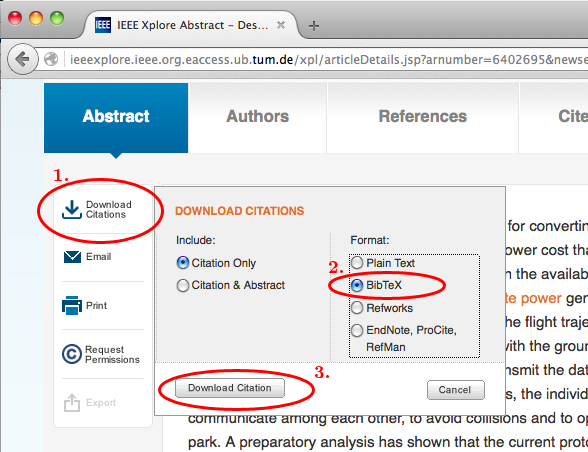
\includegraphics[width=8cm]{Images/IEEExplore.png}
	\caption{Downloading a bibtex entry from IEEExplore.}
	\label{IEEExplore.png}
\end{figure}


\subsection{Further Reading}

Please also read “How to write for Technical Periodicals \& conferences” by IEEE, \url{http://www.ieee.org/publications_standards/publications/authors/author_guide_interactive.pdf}, at least Secs.~6--7. Another guide is \url{http://journals.aps.org/files/rmpguide.pdf}.


\section{Guidelines for Your Presentation}

In the following, a few guidelines (dos and don'ts) for your presentations are given:

\begin{itemize}
	\item Do not create a bullet point-“standard” Power Point presentation.
	\item Place almost no text on the slides. Place almost no math on the slides, except one can understand quickly, and if it helps to illustrate your idea.
	\item Instead use images and graphs, with which you tell a story and sketch your idea. A story teller does not need to draw an outline at the beginning of the story.
	\item Place affiliation, dates, logos etc.\ only on the first slide (title slide). On all other slides, place only a slide number and do note place other boarders. Use a single color background, e.g.\ just black or white.
	\item Do not overload your slides.
	\item Use a similar structure as in your report/thesis: title, motivation incl.\ previous/related works, your approach/idea, your results, conclusions, outlook.
	\item Rehearse your presentation several times. Make sure, you are $\unit[\pm 3]{min}$ maximum within the set time limit. You usually need about $\unit[1]{min}$ per slide.
	\item Create your presentation with only one target: The audience shall understand your key idea. Mathematical details etc.\ can be found in your report/thesis.
	\item Orient your presentation on good presentations, e.g.: Al Gore: “An Inconvenient Truth”, movie, part: \url{https://www.youtube.com/watch?v=7Q2NfEmOjug}, TED talks, \url{http://www.ted.com/} (e.g.\ \url{http://www.ted.com/talks/david_pogue_says_simplicity_sells.html}, \url{http://www.ted.com/talks/shai_agassi_on_electric_cars.html}), Apple keynotes by Steve Jobs, PresentationZen, \url{http://www.presentationzen.com/}.
\end{itemize}





\ifthenelse{\boolean{isIEEETemplate} \OR \boolean{isArticleTemplate}}{
	\section*{Acknowledgments}
	
	\dots if you would like to thank someone. In a thesis, acknowledgements are usually put on one of the first pages.
}{}




% Can use something like this to put references on a page
% by themselves when using endfloat and the captionsoff option.
\ifCLASSOPTIONcaptionsoff
  \newpage
\fi



% trigger a \newpage just before the given reference
% number - used to balance the columns on the last page
% adjust value as needed - may need to be readjusted if
% the document is modified later
%\IEEEtriggeratref{8}
% The "triggered" command can be changed if desired:
%\IEEEtriggercmd{\enlargethispage{-5in}}

% references section

\ifthenelse{\boolean{isIEEETemplate} \OR \boolean{isArticleTemplate}}{
	\bibliographystyle{IEEEtran}
	\bibliography{IEEEabrv,GuidelinesStudentsReportsAndThesesBibliography}
}{
	\chapter*{Bibliography}
	\addcontentsline{toc}{chapter}{Bibliography}
	
%	\noindent\textit{Direct citations are marked by citation marks (“\dots”) except if the citation is a number. For those citations, the corresponding reference marks (in square brackets, [\dots]) are placed straight behind. Indirect citations are marked by reference marks as follows: Reference marks before a full stop relate to the sentence. Reference marks behind a full stop relate to everything before that reference mark up to the last reference mark of an indirect citation or the beginning of the paragraph. If direct citations are not echoed exactly, changes are marked inside square brackets.}
	
	\begingroup
	\renewcommand{\chapter}[2]{}%
	
	\bibliographystyle{unsrt}
	\bibliography{GuidelinesStudentsReportsAndThesesBibliography}
}{


\end{document}
